\clearpage
\section{ВВЕДЕНИЕ}
Наиболее распространённый метод изображения любого объекта в трёхмерных компьютерных играх --- отрисовка набора треугольников, проецируемых из виртуального трёхмерного пространства на экран.
Такой набор треугольников называется ,,мешем`` --- транслитерация устоявшегося английского термина mesh, обычно меш задаёт приближение поверхности объекта.
Целевые платформы компьютерных игр, компьютеры и игровые приставки, оснащены видеокартами --- сопроцессорами, аппаратно поддерживающими быструю отрисовку мешей.

На рисунках~\ref{fig:mesh-example-wireframe} и~\ref{fig:mesh-example-solid} приведён пример меша в виде рёбер треугольников и самих треугольников соответственно.

\begin{figure}[H]
    \centering
    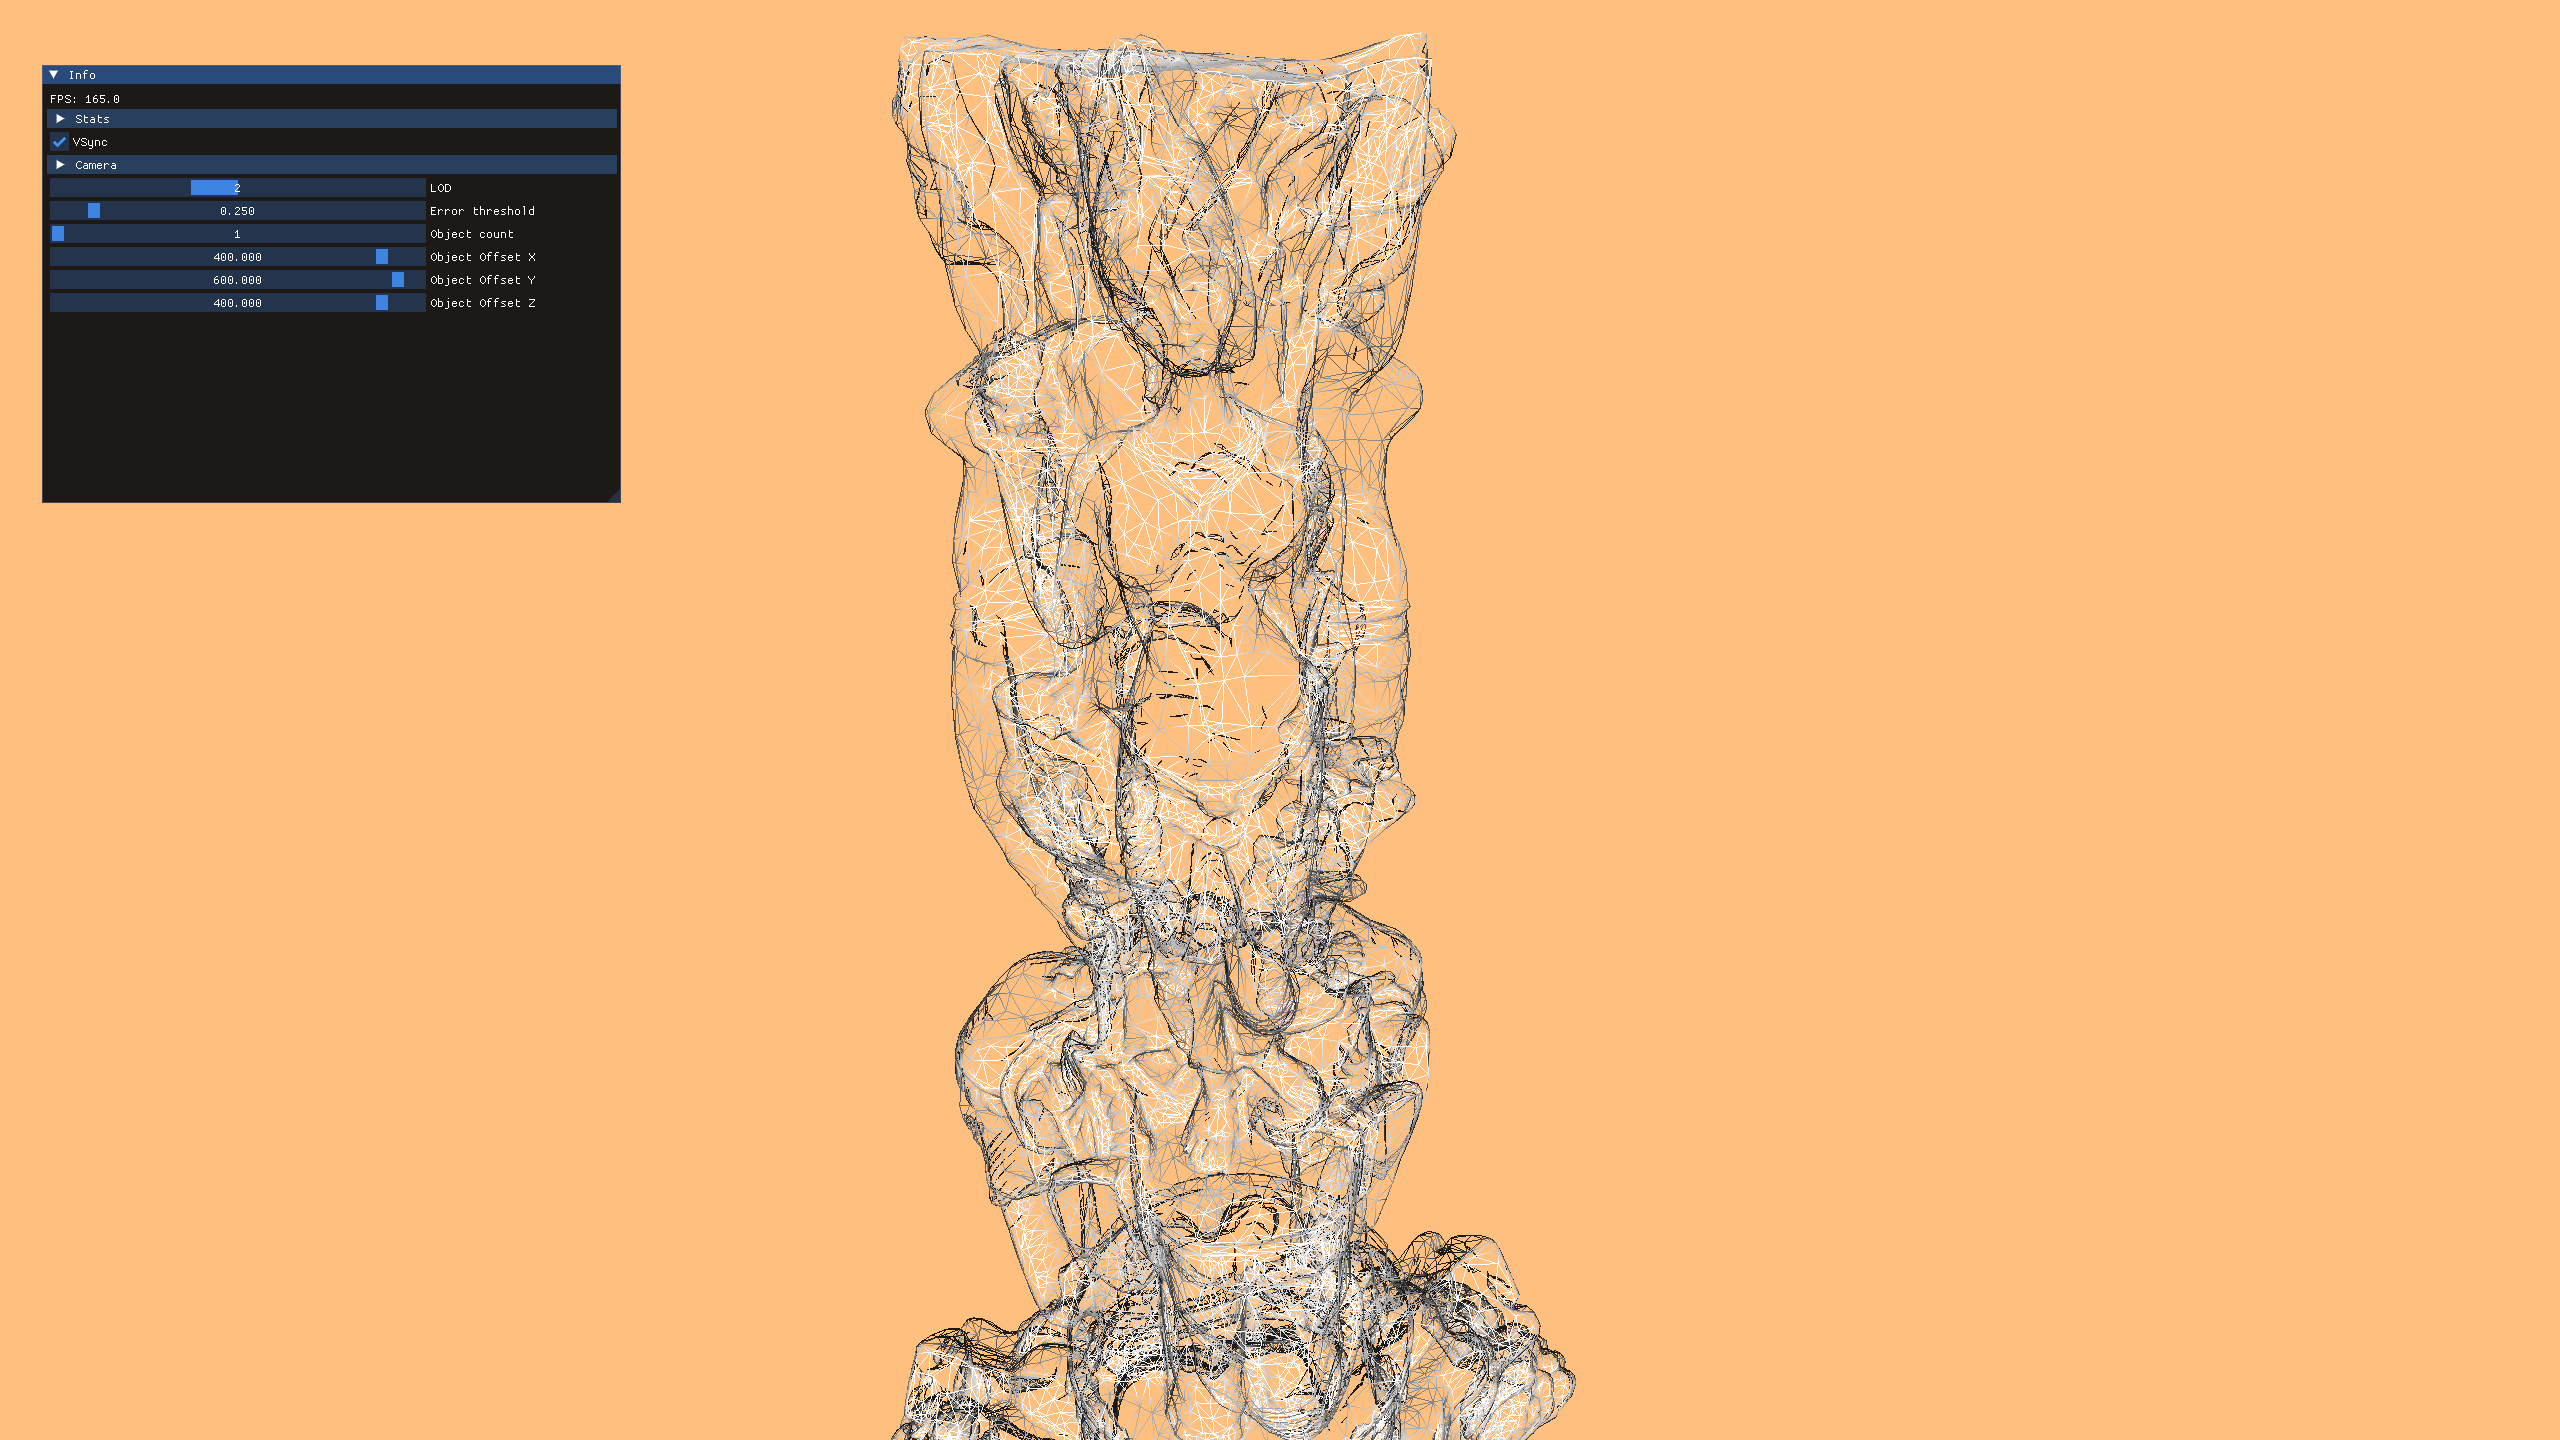
\includegraphics[width=\textwidth]{pics/mesh-example-wireframe.png}
    \caption{Пример меша}
    \label{fig:mesh-example-wireframe}
\end{figure}

\begin{figure}[H]
    \centering
    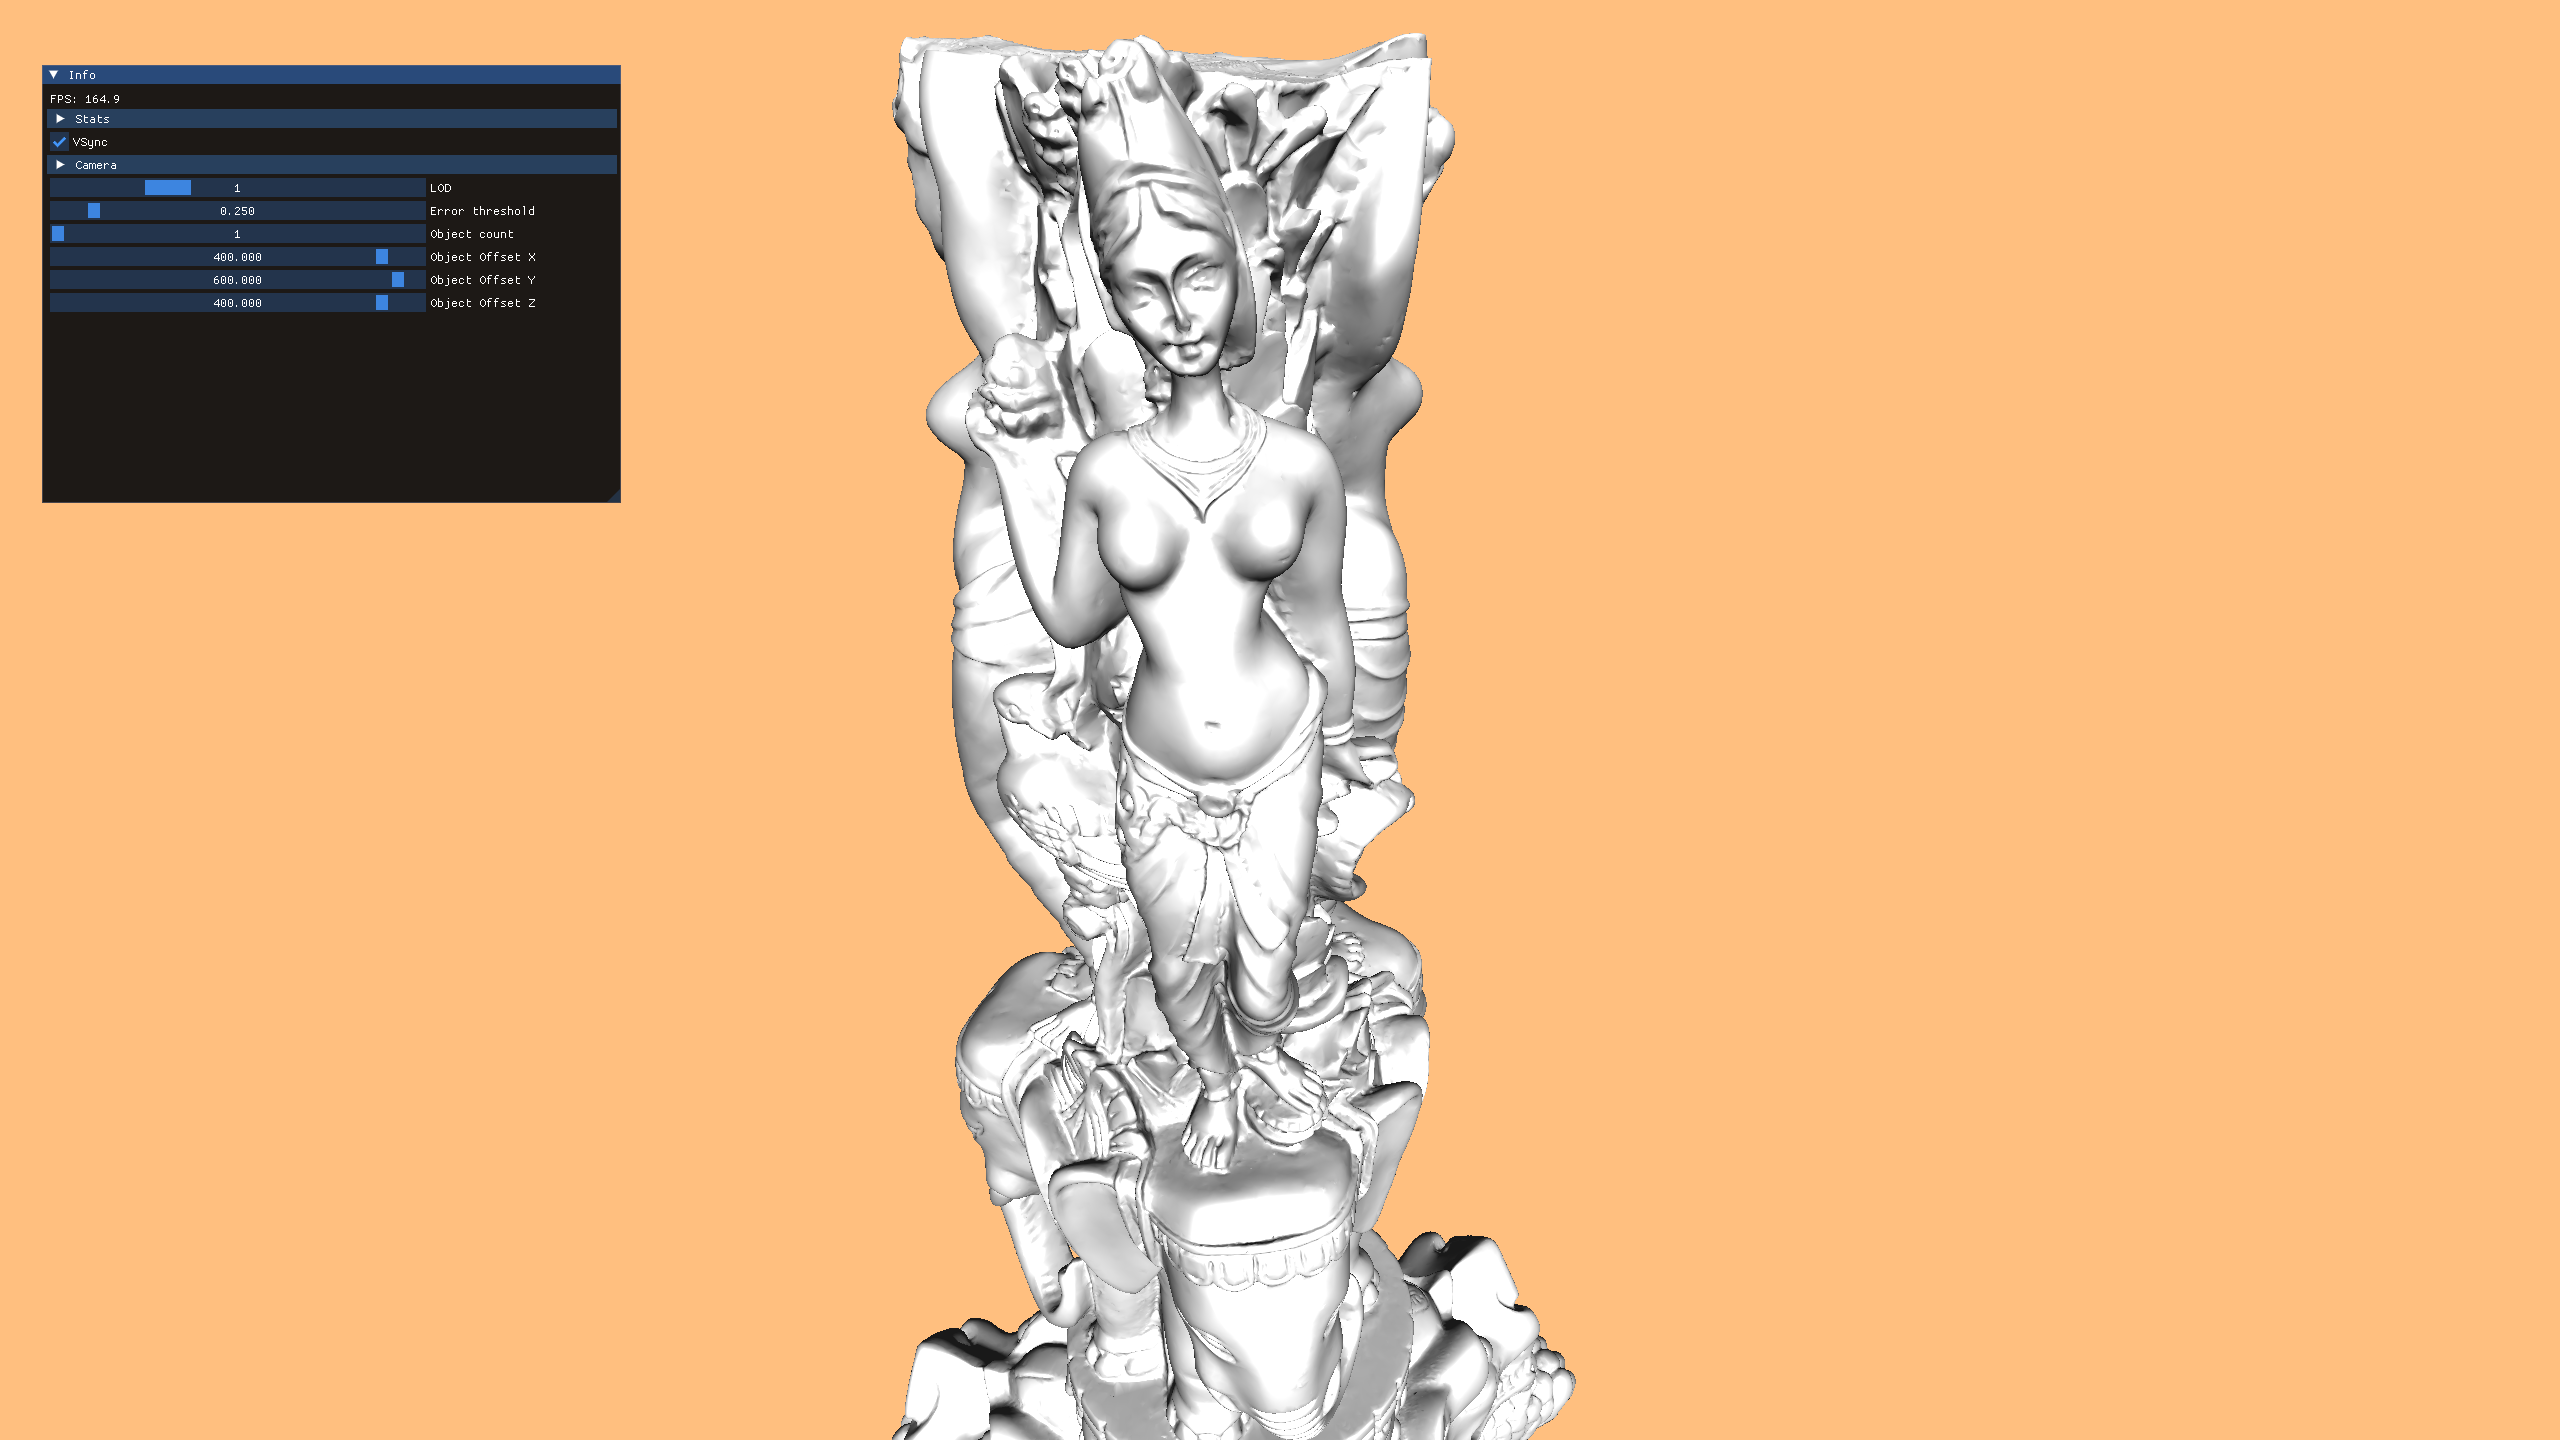
\includegraphics[width=\textwidth]{pics/mesh-example-solid.png}
    \caption{Пример меша}
    \label{fig:mesh-example-solid}
\end{figure}

Для большей правдоподобности изображения компьютерные игры стремятся увеличивать разрешение мешей --- приближать поверхность объекта большим количеством треугольников малого размера.
Во многих случаях меши, применяемые в программе, составляются из исходных мешей высокого разрешения, например, отсканированных реальных объектов.

Для компьютерных игр критически важно выводить изображение в реальном времени, т.к. оно является реакцией на пользовательский ввод.
Вычислительных мощностей современных видеокарт хватает, чтобы выводить на экран в реальном времени достаточно ограниченное количество треугольников, например, в игре Space Marine 2 от Saber Interactive на Xbox Series S за один кадр отрисовывается от 5 до 15 млн. треугольников в зависимости от сложности сцены.
Как правило, один объект не будет превышать такого порога, но в области видимости могут находиться сотни объектов одновременно, и если каждый из них содержит несколько миллионов треугольников, то отрисовывать их в реальном времени будет невозможно.

Классическое решение вышеупомянутой проблемы состоит в отрисовке объектов с разными уровнями детализации.
Уровни детализации, также называемые ,,лодами`` от английской аббревиатуры LOD (level of detail) --- это набор мешей одного и того же объекта в разных разрешениях.
Уровень детализации для отрисовки объекта выбирается на основании оценки визуального искажения данного уровня детализации с учётом положения объекта относительно камеры.
Например, для объекта, расположенного вплотную к камере, будет отрисован меш в максимальном разрешении, а для объекта далеко от камеры можно использовать низкий уровень детализации.
Такое решение далее в работе будет называться монолитным лоддированием или монолитной детализацией.

У алгоритмов, использующих уровни детализации, есть значительные проблемы: создание лодов требует ручной доработки, а подбор порогов переключения между лодами выполняется вручную.
Также существуют крупные объекты, такие как статуи, скалы и здания, для которых выбор уровня детализации неоднозначен, например, если игрок рассматривает кирпичную стену здания вблизи, то ему должны быть видны мельчайшие детали вплоть до царапин на кирпичах, но для этого здание целиком нужно рисовать в максимальном разрешении, включая ту часть стены, которая находится от игрока на таком расстоянии, что отдельные кирпичи будут едва различимы --- это требует столько же ресурсов, как если бы были видны мельчайшие детали всей стены целиком.

Существуют разные технологии, решающие проблему уменьшения вычислительной сложности отрисовки геометрии.
Помимо алгоритмов на основе уровней детализации наиболее примечательны следующие:
\begin{itemize}
    \item Geometry Clipmaps~\cite{GPUGems2GeometryClipmaps}
    \item Sparse Voxel Octrees~\cite{SparseVoxelOctrees}
    \item Nanite~\cite{NaniteManual}
\end{itemize}

Geometry Clipmaps оптимизирует отрисовку ландшафта, используя карту высот --- растровое двумерное изображение, цвет каждого пикселя в котором соответствует некоторой высоте.
Ландшафты составляют значительную часть геометрии сцены, и Geometry Clipmaps существенно ускоряют их отрисовку, но для большинства объектов невозможно составить такую карту высот в некоторой параллельной проекции, которая однозначно описывала бы всю поверхность объекта, поэтому применение этой технологии ограничено.

Sparse Voxel Octrees вместо описания поверхности объекта, которым является меш, использует описание объёма, приближая его элементарными единицами объёма --- вокселями.
Воксели являются кубическими ячейками трёхмерной сетки с малым шагом, например, 100~мкм.
Иллюстрация Sparse Voxel Octree~\cite{WikipediaSparseVoxelOctreeExample} приведена на рисунке~\ref{fig:SVO-voxel-snowman-slice-01}.

\begin{figure}[H]
    \centering
    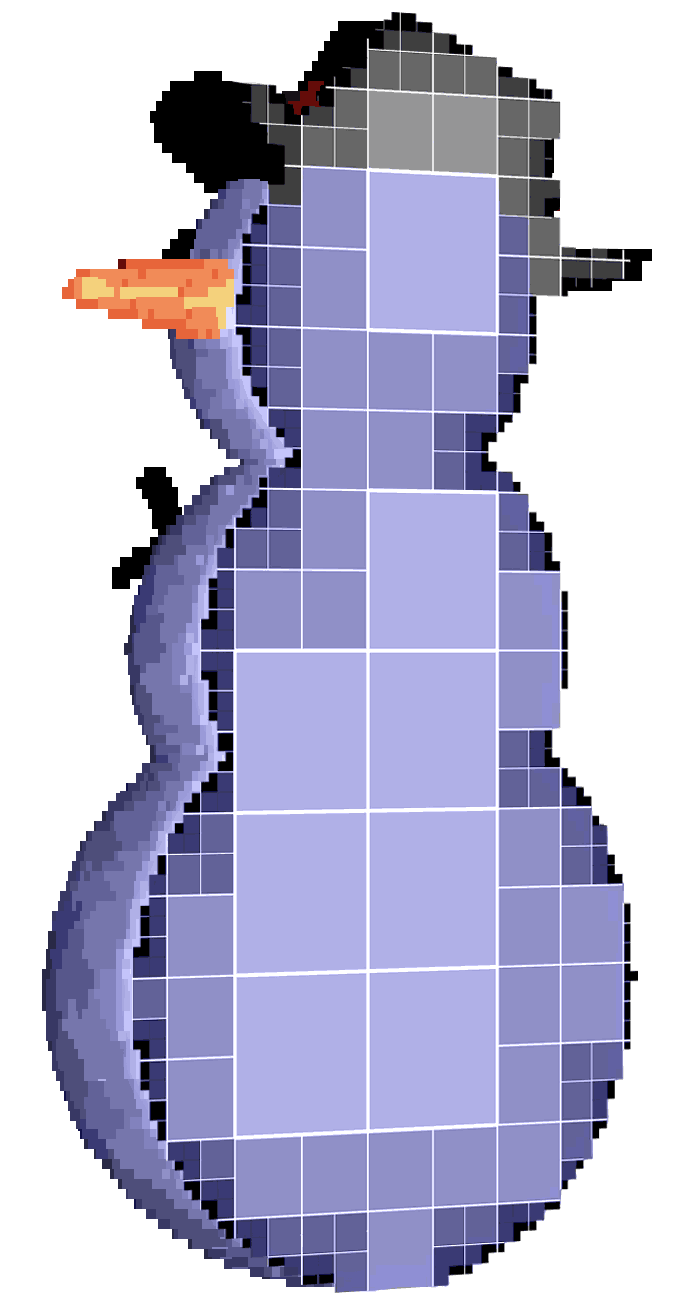
\includegraphics[width=5cm]{pics/SVO-voxel-snowman-slice-01.png}
    \caption{Срез Sparse Voxel Octree}
    \label{fig:SVO-voxel-snowman-slice-01}
\end{figure}

Основным недостатком Sparse Voxel Octrees является существенная потеря детализации по сравнению с мешами при условии сравнимого размера сжатой записи.

В 2020 году компания Epic Games представила свой подход к уменьшению сложности вычислений при отрисовке высокодетализированных объектов --- технологию Nanite в движке Unreal Engine~5.
Nanite --- технология процедурного кластерного видозависимого изменения детализации, то есть:
\begin{itemize}
    \item Nanite автоматически создаёт уровни детализации, без необходимости дорабатывать их вручную;
    \item Nanite отображает части одного объекта с разными подходящими уровнями детализации;
    \item Nanite делает швы между разными уровнями детализации незаметными;
    \item Nanite использует меш максимально возможного разрешения, для которого хватает разрешения экрана и разрешения исходного меша.
\end{itemize}

Несмотря на заявленные преимущества и то, что исходный код Nanite открыт, подобную технологию на момент написания работы в 2024 году не внедрила ни одна из ведущих компаний, таких как:
\begin{itemize}
    \item Unity
    \item Activision
    \item Ubisoft
    \item Crytek
    \item CD Projekt Red
    \item и т.д.
\end{itemize}
Epic Games остаётся единственной компанией, успешно внедрившей технологию процедурного кластерного видозависимого изменения детализации.
Следовательно, у технологии есть какие-то существенные ограничения, сравнимые с преимуществами.

Целью выпускной квалификационной работы является демонстрация технологии процедурного кластерного видозависимого лоддирования и определение её ограничений.

Для достижения этой цели поставлены следующие задачи:
\begin{enumerate}
    \item изучить механизм работы Nanite;
    \item реализовать упрощённую систему процедурного кластерного видозависимого изменения детализации
    \begin{itemize}
        % \item одна из гипотез --- Nanite очень сложен в реализации, для её проверки предлагается реализовать упрощённую версию;
        \item упрощённая версия позволит проводить объяснимые сравнения с классической реализацией;
    \end{itemize}
    \item определить проблемы, возникающие при реализации;
    \item определить принципиальные ограничения технологии;
    \item сравнить с монолитной детализацией.
\end{enumerate}

Информация о технических и принципиальных ограничениях позволит Saber Interactive принять решение о реализации полной версии технологии и интеграции в существующий движок.
